\documentclass[12pt,twoside]{article}
\usepackage[dvipsnames]{xcolor}
\usepackage{tikz,graphicx,amsmath,amsfonts,amscd,amssymb,bm,cite,epsfig,epsf,url}
\usepackage[hang,flushmargin]{footmisc}
\usepackage[colorlinks=true,urlcolor=blue,citecolor=blue]{hyperref}
\usepackage{amsthm,multirow,wasysym,appendix}
\usepackage{array,subcaption} 
% \usepackage[small,bf]{caption}
\usepackage{bbm}
\usepackage{pgfplots}
\usetikzlibrary{spy}
\usepgfplotslibrary{external}
\usepgfplotslibrary{fillbetween}
\usetikzlibrary{arrows,automata}
\usepackage{thmtools}
\usepackage{blkarray} 
\usepackage{textcomp}
\usepackage[left=0.8in,right=1.0in,top=1.0in,bottom=1.0in]{geometry}

\usepackage{times}
\usepackage{amsfonts}
\usepackage{amsmath}
\usepackage{latexsym}
\usepackage{color}
\usepackage{graphics}
\usepackage{enumerate}
\usepackage{amstext}
\usepackage{blkarray}
\usepackage{url}
\usepackage{epsfig}
\usepackage{bm}
\usepackage{hyperref}
\hypersetup{
    colorlinks=true,
    linkcolor=blue,
    filecolor=magenta,      
    urlcolor=blue,
}
\usepackage{textcomp}
\usepackage[left=0.8in,right=1.0in,top=1.0in,bottom=1.0in]{geometry}
\usepackage{mathtools}
\usepackage{minted}


%% Probability operators and functions
%
% \def \P{\mathrm{P}}
\def \P{\mathrm{P}}
\def \E{\mathrm{E}}
\def \Var{\mathrm{Var}}
\let\var\Var
\def \Cov {\mathrm{Cov}} \let\cov\Cov
\def \MSE {\mathrm{MSE}} \let\mse\MSE
\def \sgn {\mathrm{sgn}}
\def \R {\mathbb{R}}
\def \C {\mathbb{C}}
\def \N {\mathbb{N}}
\def \Z {\mathbb{Z}}
\def \cV {\mathcal{V}}
\def \cS {\mathcal{S}}
\DeclareMathOperator*{\argmin}{arg\,min}
\DeclareMathOperator*{\argmax}{arg\,max}
\newcommand{\red}[1]{\textcolor{red}{#1}}
\newcommand{\blue}[1]{\textcolor{blue}{#1}}
\newcommand{\green}[1]{\textcolor{ForestGreen}{ #1}}
\newcommand{\fuchsia}[1]{\textcolor{RoyalPurple}{ #1}}

%
%% Probability distributions
%
%\def \Bern    {\mathrm{Bern}}
%\def \Binom   {\mathrm{Binom}}
%\def \Exp     {\mathrm{Exp}}
%\def \Geom    {\mathrm{Geom}}
%\def \Norm    {\mathcal{N}}
%\def \Poisson {\mathrm{Poisson}}
%\def \Unif    {\mathrm {U}}
%
\newcommand{\bdb}[1]{\textcolor{red}{#1}}

\newcommand{\ml}[1]{\mathcal{ #1 } }
\newcommand{\wh}[1]{\widehat{ #1 } }
\newcommand{\wt}[1]{\widetilde{ #1 } }
\newcommand{\conj}[1]{\overline{ #1 } }
\newcommand{\rnd}[1]{\tilde{ #1 } }
\newcommand{\rv}[1]{ \rnd{ #1}  }
\newcommand{\rx}{\rnd{ x}  }
\newcommand{\ry}{\rnd{ y}  }
\newcommand{\ra}{\rnd{ a}  }
\newcommand{\rb}{\rnd{ b}  }
\newcommand{\rpc}{\widetilde{ pc}  }

\def \cnd {\, | \,}
\def \Id { I }
\def \J {\mathbf{1}\mathbf{1}^T}

\newcommand{\op}[1]{\operatorname{#1}}
\newcommand{\setdef}[2]{ := \keys{ #1 \; | \; #2 } }
\newcommand{\set}[2]{ \keys{ #1 \; | \; #2 } }
\newcommand{\sign}[1]{\op{sign}\left( #1 \right) }
\newcommand{\trace}[1]{\op{tr}\left( #1 \right) }
\newcommand{\tr}[1]{\op{tr}\left( #1 \right) }
\newcommand{\inv}[1]{\left( #1 \right)^{-1} }
\newcommand{\abs}[1]{\left| #1 \right|}
\newcommand{\sabs}[1]{| #1 |}
\newcommand{\keys}[1]{\left\{ #1 \right\}}
\newcommand{\sqbr}[1]{\left[ #1 \right]}
\newcommand{\sbrac}[1]{ ( #1 ) }
\newcommand{\brac}[1]{\left( #1 \right) }
\newcommand{\bbrac}[1]{\big( #1 \big) }
\newcommand{\Bbrac}[1]{\Big( #1 \Big)}
\newcommand{\BBbrac}[1]{\BIG( #1 \Big)}
\newcommand{\MAT}[1]{\begin{bmatrix} #1 \end{bmatrix}}
\newcommand{\sMAT}[1]{\left(\begin{smallmatrix} #1 \end{smallmatrix}\right)}
\newcommand{\sMATn}[1]{\begin{smallmatrix} #1 \end{smallmatrix}}
\newcommand{\PROD}[2]{\left \langle #1, #2\right \rangle}
\newcommand{\PRODs}[2]{\langle #1, #2 \rangle}
\newcommand{\der}[2]{\frac{\text{d}#2}{\text{d}#1}}
\newcommand{\pder}[2]{\frac{\partial#2}{\partial#1}}
\newcommand{\derTwo}[2]{\frac{\text{d}^2#2}{\text{d}#1^2}}
\newcommand{\ceil}[1]{\lceil #1 \rceil}
\newcommand{\Imag}[1]{\op{Im}\brac{ #1 }}
\newcommand{\Real}[1]{\op{Re}\brac{ #1 }}
\newcommand{\norm}[1]{\left|\left| #1 \right|\right| }
\newcommand{\norms}[1]{ \| #1 \|  }
\newcommand{\normProd}[1]{\left|\left| #1 \right|\right| _{\PROD{\cdot}{\cdot}} }
\newcommand{\normTwo}[1]{\left|\left| #1 \right|\right| _{2} }
\newcommand{\normTwos}[1]{ \| #1  \| _{2} }
\newcommand{\normZero}[1]{\left|\left| #1 \right|\right| _{0} }
\newcommand{\normTV}[1]{\left|\left| #1 \right|\right|  _{ \op{TV}  } }% _{\op{c} \ell_1} }
\newcommand{\normOne}[1]{\left|\left| #1 \right|\right| _{1} }
\newcommand{\normOnes}[1]{\| #1 \| _{1} }
\newcommand{\normOneTwo}[1]{\left|\left| #1 \right|\right| _{1,2} }
\newcommand{\normF}[1]{\left|\left| #1 \right|\right| _{\op{F}} }
\newcommand{\normLTwo}[1]{\left|\left| #1 \right|\right| _{\ml{L}_2} }
\newcommand{\normNuc}[1]{\left|\left| #1 \right|\right| _{\ast} }
\newcommand{\normOp}[1]{\left|\left| #1 \right|\right|  }
\newcommand{\normInf}[1]{\left|\left| #1 \right|\right| _{\infty}  }
\newcommand{\proj}[1]{\mathcal{P}_{#1} \, }
\newcommand{\diff}[1]{ \, \text{d}#1 }
\newcommand{\vc}[1]{\boldsymbol{\vec{#1}}}
\newcommand{\rc}[1]{\boldsymbol{#1}}
\newcommand{\vx}{\vec{x}}
\newcommand{\vy}{\vec{y}}
\newcommand{\vz}{\vec{z}}
\newcommand{\vu}{\vec{u}}
\newcommand{\vv}{\vec{v}}
\newcommand{\vb}{\vec{\beta}}
\newcommand{\va}{\vec{\alpha}}
\newcommand{\vaa}{\vec{a}}
\newcommand{\vbb}{\vec{b}}
\newcommand{\vg}{\vec{g}}
\newcommand{\vw}{\vec{w}}
\newcommand{\vh}{\vec{h}}
\newcommand{\vnu}{\vec{\nu}}
\newcommand{\rvnu}{\vc{\nu}}

\newtheorem{theorem}{Theorem}[section]
% \declaretheorem[style=plain,qed=$\square$]{theorem}
\newtheorem{corollary}[theorem]{Corollary}
\newtheorem{definition}[theorem]{Definition}
\newtheorem{lemma}[theorem]{Lemma}
\newtheorem{remark}[theorem]{Remark}
\newtheorem{algorithm}[theorem]{Algorithm}

% \theoremstyle{definition}
%\newtheorem{example}[proof]{Example}
%\declaretheorem[style=definition,qed=$\triangle$,sibling=definition]{example}
%\declaretheorem[style=definition,qed=$\bigcirc$,sibling=definition]{application}

%
%% Typographic tweaks and miscellaneous
%\newcommand{\sfrac}[2]{\mbox{\small$\displaystyle\frac{#1}{#2}$}}
%\newcommand{\suchthat}{\kern0.1em{:}\kern0.3em}
%\newcommand{\qqquad}{\kern3em}
%\newcommand{\cond}{\,|\,}
%\def\Matlab{\textsc{Matlab}}
%\newcommand{\displayskip}[1]{\abovedisplayskip #1\belowdisplayskip #1}
%\newcommand{\term}[1]{\emph{#1}}
%\renewcommand{\implies}{\;\Rightarrow\;}

% My macros

\def\Kset{\mathbb{K}}
\def\Nset{\mathbb{N}}
\def\Qset{\mathbb{Q}}
\def\Rset{\mathbb{R}}
\def\Sset{\mathbb{S}}
\def\Zset{\mathbb{Z}}
\def\squareforqed{\hbox{\rlap{$\sqcap$}$\sqcup$}}
\def\qed{\ifmmode\squareforqed\else{\unskip\nobreak\hfil
\penalty50\hskip1em\null\nobreak\hfil\squareforqed
\parfillskip=0pt\finalhyphendemerits=0\endgraf}\fi}

%\DeclareMathOperator*{\E}{\rm E}
%\DeclareMathOperator*{\argmax}{\rm argmax}
%\DeclareMathOperator*{\argmin}{\rm argmin}
%\DeclareMathOperator{\sgn}{sign}
\DeclareMathOperator{\supp}{supp}
\DeclareMathOperator{\last}{last}
%\DeclareMathOperator{\sign}{\sgn}
\DeclareMathOperator{\diag}{diag}
\providecommand{\abs}[1]{\lvert#1\rvert}
\providecommand{\norm}[1]{\lVert#1\rVert}
\def\vcdim{\textnormal{VCdim}}
\DeclareMathOperator*{\B}{\textbf{B}}

%\DeclarePairedDelimiter\ceil{\lceil}{\rceil}
%\DeclarePairedDelimiter\floor{\lfloor}{\rfloor}

\newcommand{\cX}{{\mathcal X}}
\newcommand{\cY}{{\mathcal Y}}
\newcommand{\cA}{{\mathcal A}}
\newcommand{\ignore}[1]{}
\newcommand{\bi}{\begin{itemize}}
\newcommand{\ei}{\end{itemize}}
\newcommand{\be}{\begin{enumerate}}
\newcommand{\ee}{\end{enumerate}}
\newcommand{\bd}{\begin{description}}
\newcommand{\ed}{\end{description}}
\newcommand{\h}{\widehat}
\newcommand{\e}{\epsilon}
\newcommand{\mat}[1]{{\mathbf #1}}
%\newcommand{\R}{\mat{R}}
\newcommand{\0}{\mat{0}}
\newcommand{\M}{\mat{M}}

\newcommand{\D}{\mat{D}}
\renewcommand{\r}{\mat{r}}
\newcommand{\x}{\mat{x}}
\renewcommand{\u}{\mat{u}}
\renewcommand{\v}{\mat{v}}
\newcommand{\w}{\mat{w}}
\renewcommand{\H}{\text{0}}
\newcommand{\T}{\text{1}}
%\newcommand{\set}[1]{\{#1\}}
\newcommand{\xxi}{{\boldsymbol \xi}}
\newcommand{\ssigma}{{\boldsymbol \sigma}}
\newcommand{\Alpha}{{\boldsymbol \alpha}}
\newcommand{\tts}{\tt \small}
\newcommand{\hint}{\emph{hint}}
\newcommand{\matr}[1]{\bm{#1}}     % ISO complying version
\newcommand{\vect}[1]{\bm{#1}} % vectors

%\newcommand{\Var}{\mathrm{Var}}
%\newcommand{\Cov}{\mathrm{Cov}}

% New commands
\newcommand{\SP}{\mathbf{S}_{+}^n}
\newcommand{\Proj}{\mathcal{P}_{\mathcal{S}}}
\DeclarePairedDelimiterX{\inp}[2]{\langle}{\rangle}{#1, #2}
\newtheorem{proof}{Proof}


\begin{document}

\begin{center}
{\large{\textbf{Homework 10}} } \vspace{0.2cm}\\
Due May 3 at 11 pm
\end{center}
Yves Greatti - yg390\\

\begin{enumerate}

\item (Hann window)
In this problem we analyze the Hann window in the frequency domain. 
 \begin{enumerate}
 \item Prove that for any vector $x \in \C^{N}$, if $y \in \C^{N}$ is defined as 
\begin{align}
y \,[j] := x[j] \exp \brac{\frac{i2 \pi m j}{N} },
\end{align}
for some integer $m$, then the DFT of $y$ equals $\hat{y}=\hat{x}^{\downarrow \, m}$, where $\hat{x}$ is the DFT of $x$.\\
We have
\begin{align*}
	\hat{y}[k]	&=	\sum_{j=1}^N x(j)  \exp \brac{\frac{-i2 \pi k j}{N} } \exp \brac{\frac{i2 \pi m j}{N} } \\
			&=	\sum_{j=1}^N x(j)  \exp \brac{\frac{-i2 \pi (k-m) j}{N} } \\
			&=    \hat{x}^{\downarrow \, m}[k] \\
\end{align*}

 \item The Hann window $h \in \C^{N}$ of width $2w$ equals
\begin{align}
h\sqbr{j} & :=  
 \begin{cases}
  \frac{1}{2} \brac{1 + \cos \brac{ \frac{ \pi j}{w}}} & \text{if } \abs{j} \leq w,\\
   0 & \text{otherwise.}
  \end{cases}
\end{align} 
Use the result from part (a) to show that the DFT of $h$ can be expressed as
\begin{align}
\label{eq:hann}
\hat{h} = \frac{1}{2}\hat{\pi} + \frac{1}{4}\hat{\pi}^{\downarrow \, -N/2w} + \frac{1}{4}\hat{\pi}^{\downarrow \, N/2w}.
\end{align}\\
 The rectangular window $\hat{\pi} \in  \C^{N}$ with width $2w$ is defined by
\begin{equation*}
  \hat{y}[j] =
    \begin{cases}
      1 & \text{if } \abs{j} \leq w,\\
      0 & \text{otherwise}
    \end{cases}       
\end{equation*}
For $\abs{j} \leq w$, $h\sqbr{j} =  \frac{1}{2} \brac{1 + \cos \brac{ \frac{ \pi j}{w}}} =  \brac{\frac{1}{2}  \cdot 1 +  \frac{ \exp \brac{\frac{i \pi j}{w} } 
+  \exp \brac{\frac{-i \pi j}{w} }} {2} } = \frac{1}{2}  \cdot 1  +  \frac{1}{4}  \exp \brac{\frac{i \pi j}{w} } \cdot 1 + \frac{1}{4}  \exp \brac{\frac{-i \pi j}{w} } \cdot 1$.
Using part a, with $m= \frac{N}{2w}$, the DFT of  $h$ is then $\hat{h} = \frac{1}{2}\hat{\pi} + \frac{1}{4}\hat{\pi}^{\downarrow \, -N/2w} + \frac{1}{4}\hat{\pi}^{\downarrow \, N/2w}$.


\item Plot $\hat{h}$ as well as the different components in Eq.~\eqref{eq:hann}. Interpret what you see in terms of the desired properties of a windowing function. 
\begin{figure}[H]
		\centering
		\captionsetup{justification=centering}
		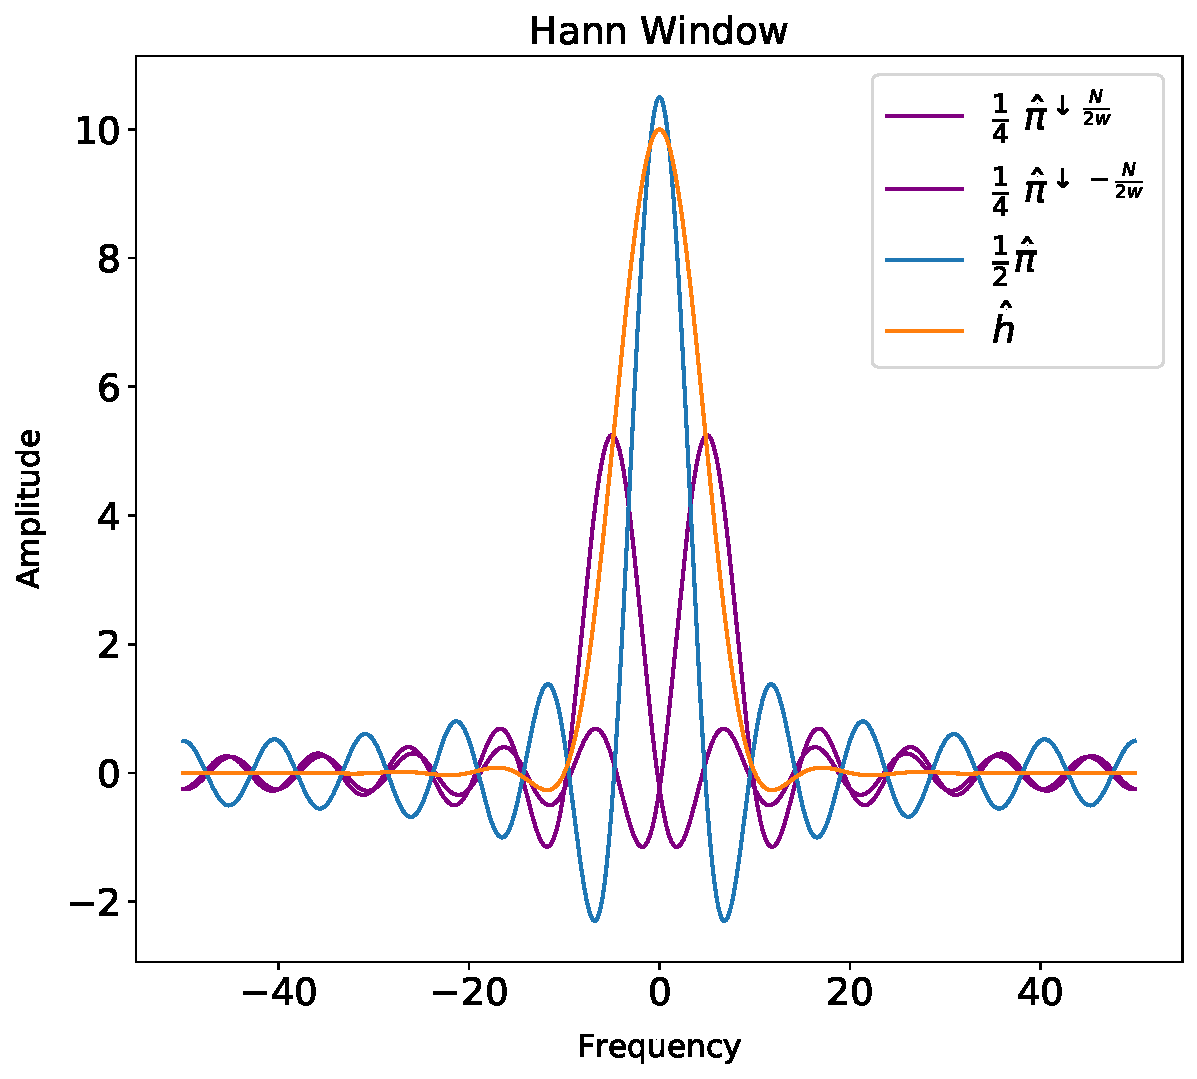
\includegraphics[width=200pt]{code/images/Hann.pdf}
		\caption{Frequency response of the Hann window}
	\end{figure}

 \end{enumerate}
  
 \newpage
 \item (STFT inverse) In this problem we show a simple way to invert the STFT.
 \begin{enumerate}
  \item In the definition of the STFT set $w_{[\ell]}$ to be a rectangular window where all entries are equal to one, and let $\alpha_{\op{ov}}=0.5$. Show that the STFT can be inverted using just two operations: applying the inverse DFT and subsampling.
  \item What is the disadvantage of using this rectangular window?
  \end{enumerate}
 
 \item (Haar wavelet) Define the discrete Haar wavelet $\mu_{2^s,p}\in\RR^{2^n}$ at scale
  $2^s$ and position $p$ by
  $$\mu_{2^s,p}[j] :=
  \begin{cases}
    -1/\sqrt{2^{s}} & \text{if $j\in\{p\cdot 2^s,p\cdot 2^s+1,\ldots,p\cdot 2^s+2^{s-1}-1\}$,}\\
    1/\sqrt{2^{s}} & \text{if $j\in\{p\cdot 2^s+2^{s-1},2^s+2^{s-1}+1,\ldots,(p+1)\cdot2^{s}-1\}$,}\\
    0 & \text{otherwise,}
  \end{cases}
  $$
  where $0<s\leq n$ and $0 \leq p \leq 2^{n-s}-1$.  Define the
  discrete Haar scaling function $\varphi_{2^s,p}\in\RR^{2^n}$ at scale $2^s$ and position $p$  by
  $$\varphi_{2^s,p}[j]=
  \begin{cases}
    1/\sqrt{2^{s}} & \text{if $j\in\{p\cdot 2^s,p\cdots 2^s+1,\ldots,(p+1)\cdot 2^{s}-1\}$,}\\
    0 & \text{otherwise,}
  \end{cases}$$
  where $0<s\leq n$ and $0\leq p\leq 2^{n-s}-1$.
  The code for this
  exercise is contained in the haar.py file. Include all generated plots in your submission.
  \begin{enumerate}
  \item Define $V_0:=\RR^{2^n}$.  For $k>0$, let $V_k\subset\RR^{2^n}$ denote the subspace
    of all vectors that are constant on segments of size $2^k$.  That
    is
    $$V_k := \{x\in\RR^{2^n}: \text{$x[i] = x[j]$ if $\lfloor
      i/2^k\rfloor = \lfloor j/2^k\rfloor$}\}.$$
    Give an orthonormal basis for $V_k$.  What is the dimension of
    $V_k$? 
  \item Fix $0\leq k < n$, and note that $V_k\supset V_{k+1}$.  Give an orthonormal basis for
    the set
    $$W_{k+1}=\{x\in V_k : \text{$\langle x,y\rangle = 0$ for all
      $y\in V_{k+1}$}\},$$
    the orthogonal complement of $V_{k+1}$ in $V_k$.  Thus
    $V_k=V_{k+1}\oplus W_{k+1}$. What is the
    dimension of $W_{k+1}$?
  \item For $1\leq k\leq n$ give an orthonormal basis for the set
    $$W_{\leq k}=\{x\in \RR^{2^n} : \text{$\langle x,y\rangle = 0$ for all
      $y\in V_{k}$}\},$$
    the orthogonal complement of $V_{k}$ in $\RR^{2^n}$.  Thus
    $\RR^{2^n}=V_{k}\oplus W_{\leq k}$. What is the
    dimension of $W_{\leq k}$?
  \item Complete the wavelet and scaling functions in \emph{haar.py} that implement $\mu$
    and $\varphi$ above, respectively.  See the comments for more
    details.
  \item Complete the projectV function that orthogonally projects a
    given vector onto $V_k$. [Hint: Consider averaging the values on each segment.]
  \item Complete the projectW function that orthogonally projects a
    given vector onto $W_k$. [Hint: You can use projectV.]
  \item Complete the function \emph{wavelet\_coeffs}
    which computes all of the (non-overlapping) wavelet 
    coefficients of a given data vector at a given scale.  
    See the comments for more details.
    \item Report the plots generated by the code, which apply your wavelet transform to some electrocardiogram data.
  \end{enumerate}

 
  \item (Denoising with the STFT)  
In the lecture, we saw that STFT often yields sparse representation for a signal but dense representation for noise. Building on this, we derived hard thresholding (Algorithm 4.1 in notes) and block thresholding (Algorithm 4.2 in notes) to denoise signals. In this question, we will denoise audio signals.  \texttt{audio\_denoising.ipynb} contains skeleton code for the task. The notebook will download required dataset and contains other utility functions for loading data, plotting and playing the audio signals. You have to fill in the functions \texttt{get\_block\_L2\_norm()} and \texttt{stft\_denoising()}. Report all the plots generated by the script.


 \end{enumerate}
\end{document}
